\chapter{Literature Review}

\section{Evolution of Time Series Forecasting} % Section 2.1


Nowadays \textbf{Time series forecasting} has become one, if not the most, crucial tool used in decision-making and strategic planning processes across a wide range of industries such as finance, economics, environmental science, and healthcare \cite{article}. The extensive use of time series analysis in many different industries can be attributed to its ability in examining past data, detecting hidden pattern, trends and seasonality and providing insightful forecasts, which is particularly important for the businesses in order to react and prepare for upcoming events. The methodologies used has changed considerably over the years thanks to the technological innovation, in  particular, the key drivers that have spurred the progress in time series analysis have been the increase of data availability and data volume, which have been pushed by the the rise of social media, Internet of Things (IoT), and multimedia, along with the growth of cloud computing, a powerful technology that enables to perform massive-scale and complex computing eliminating the need to purchase and maintain expensive computing hardware, dedicated space, and software\cite{HASHEM201598}.
The history of time series analysis goes back to the late 19th century, with the foundational work of Francis Galton and Karl Pearson on correlation, which then posed the basis for \textbf{George Udny Yule}, a British statistician, to further advance this concepts, developing the idea of regression between two variables X and Y, without relying on the assumption that the two variables were jointly normally distributed \cite{l_kristensen_foundations_2021} and its first known application was in his 1927 with the analysis of sunspots \cite{SILVERMAN198899}, in this paper Yule developed what is now known as an autoregressive time series analysis in order to estiamate the number of sunsposts for a given year as a function of the sunspots of the two preceding years and a presumed random disturbance. This fist model was a building block for the \textbf{ARIMA} (Autoregressive Integrated Moving Average) model, later developed in the 1970s by two mathematicians, George Box and Gwilym Jenkins, in a publication called "Time Series Analysis: Forecasting and Control", with the objective of capturing the underlying patterns in time series data leveraging the three components that compose the model: autoregression, integrated, moving average. \cite{article_2}. The ARIMA model has gained a lot of popularity in the past and was one of the most commonly used approach to time series modeling as they take both long-term trends and sudden shocks into account, and many different variations where developed, to deal with the limitations of the original one, namely the ARIMAX, SARIMA, SARIMAX, VARIMA and VARIMAX models. In modern times, although ARIMA models are still being used, they are considered "classical" approaches and with the technological and statistical advancement new techniques and algorithms have been developed, capable of handling more complexed, high-dimensional, non linear time series data, leveraging machine learning and deep leaning models.


\subsection{Classical Models (ARIMA, SARIMA, GARCH)} % Subsection 2.1.1
\subsubsection{ARIMA models}
An \textbf{ARIMA} (Autoregressive Integrated Moving Average) model, it's a more sophisticated extension of the simpler \textbf{ARMA} (Auto Regressive Moving Average) model, which combines two concepts: AR (Auto Regressive) and MA (Moving Average). 

\textbf{AR model}

Autoregressive models are regression models applied on lag series generated using the original time series. In mulitivariate linear regression, the output, the dependendent variable, is expressed as linear combination of multiple independent variables: \( y = \beta_0 + \beta_1 x_1 + \beta_2 x_2 + \cdots + \beta_n x_n + \epsilon \).
Similarly in autoregressive models with p lags or an \textbf{AR(p)} models the output (the future data point) can be expressed as a linear combination of the past p data points, where p represent the lag window: 
\begin{equation}
 y_t = \phi_1 y_{t-1} + \phi_2 y_{t-2} + \cdots + \phi_p y_{t-p} + \epsilon_t 
\end{equation}
Autoregressive models, in order to be applied, require time series to be \textbf{stationary}, which means that the statistical properties of the series, such as its mean, variance, and auto-covariance, remain constant over time. Otherwise non-stationary data can lead to unreliable model outputs and inaccurate predictions. Practically this imposes certain restrictions on the values of the autoregressive coefficients, which implies that the roots of the characteristic equation:
\begin{equation}
 1 - \phi_1 z - \phi_2 z^2 - \ldots - \phi_p z^p = 0
\end{equation}
must lie outside the unit circle, (\(|z_i| > 1 \quad\)for all roots \(z_i)\)) \cite[Section 3.2]{box1970time}.

\begin{figure}[H]
    \centering
    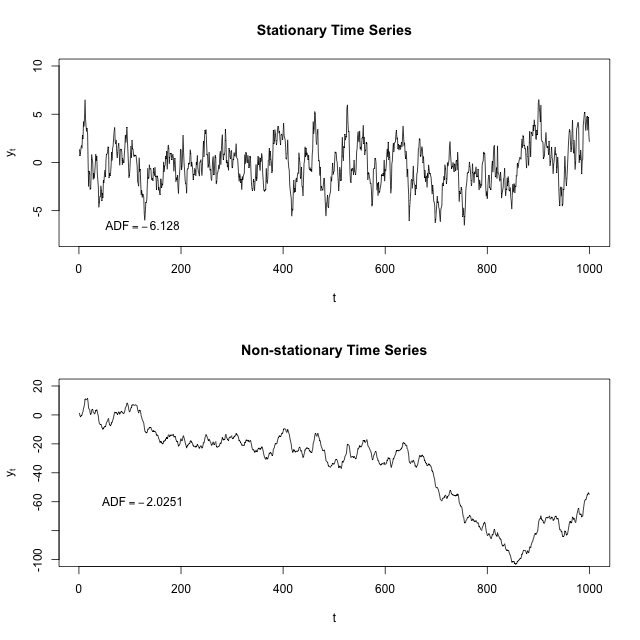
\includegraphics[width=0.50\textwidth]{Machine_learning_thesis/Images/Stationarycomparison.png}
    \caption{Example of a stationary and non-stationary process.} 
    \label{fig:Stationarycomparison}
\end{figure}

\textbf{MA model}

A moving average model uses past forecast errors in a regression-like model to predict an output(future data point), in particular, in a moving average model of order q, \textbf{MA(q)}, the ‘q’ parameter represents the number of lagged error terms to be considered in the model equation:
\begin{equation}
y_t = \mu + \varepsilon_t + \theta_1 \varepsilon_{t-1} + \theta_2 \varepsilon_{t-2} + \cdots + \theta_q \varepsilon_{t-q}
\label{MA equation}
\end{equation}
Contrary to AR(p) models, MA(q) models are stationary for any values of the coefficients \cite{chatfield2009}, indeed, if we consider the equation of a MA(q) model \eqref{MA equation}, \(y_t\) is essentially a linear combination of present and past values of \(\varepsilon_{t}\), which are assumed to be independent and identically distributed random variables with mean of zero and constant variance \( \sigma^2\), whose terms are uncorrelated. Nevertheless some constraints on the parameters of the models should be applied anyway to ensure that the model is \textbf{invertible}, which means that it can be algebraically equivalent to a converging infinite order AR model, AR(\(\infty\)), this ensure that it exists a unique MA process for a given autocorrelation function \cite{chatfield2009}. Practically this is achieved if the roots of the characteristic equation: 
\begin{equation}
 1 - \phi_1 z - \phi_2 z^2 - \ldots - \phi_p z^p = 0
\end{equation}
all lies outside the unit circle,(\(|z_i| > 1 \quad\)for all roots \(z_i)\)) \cite[pag. 50] {box1970time}.

\textbf{ARMA model}

An \textbf{ARMA(p,q)} model simply merges the two previously described models, therefore it can be expressed as: 
\begin{equation}
y_t = \mu + \phi_1 y_{t-1} + \theta_1 \epsilon_{t-1} + \epsilon_t
\end{equation}
where p and q are respectivelly the orders of the AR and MA models.

\textbf{ARIMA model}

In practise, the majority of real world time series are not stationary, and thus they must often be transformed in order to make them stationary. An \textbf{ARIMA(p, q, d)} model it's a generalizations of the autoregressive moving average (ARMA) model to non-stationary series and periodic variation with the addition of an integration component, denoted with \textbf{I(d)}, which helps  remove trends and stabilize the series in the mean sense (but it does not affect the non-stationarity of the variance or autocovariance) \cite{chatfield2009}. This can be done by differencing, which involves subtracting the preceding observation from the current one, mathematically:
\begin{equation}
 y'_t = y_t - y_{t-1}
\end{equation}
This operation is known as "first differencing",  \(\Delta\), and it is often sufficient to eliminate linear trends and achieve stationarity. If the series still shows trends or non-stationary behavior after the first pass through this process, applying "second differencing", \(\Delta^2\), may help. 
\begin{equation}
 y_t'' = (y_t - y_{t-1}) - (y_{t-1} - y_{t-2}) = y_t - 2y_{t-1} + y_{t-2}
\end{equation}
The total number of differencing is determined by the parameter d, which typically assumes the values 0, 1, 2 as higher differencing can remove too much informations from the data, over-complicating the model. The generalized  ARIMA (Autoregressive Integrated Moving Average) model can be expressed mathematically as \cite{Hung2023}: 
\begin{equation}
y_t = c + \phi_1 y_{t-1} + \cdots + \phi_p y_{t-p} + \theta_1 \epsilon_{t-1} + \cdots + \theta_q \epsilon_{t-q} + \epsilon_t
\label{ARIMA equation}
\end{equation}
which can be rewritten using backshift notation as:
\begin{equation}
\Phi(B^d)(y_t - \mu) = \Theta(B)\epsilon_t
\end{equation}
where: 
\begin{itemize}

    \item \( B \) is the backshift operator such that \( B^k y_t = y_{t-k} \).
    \item \( \Phi(B^d) \) is the autoregressive polynomial of order \( p \) given by: \(\Phi(B^d) = 1 - \phi_1 B - \phi_2 B^2 - \ldots - \phi_p B^p\)
    \item \( \Theta(B) \) is the moving average polynomial of order \( q \) given by: \(\Theta(B) = 1 + \theta_1 B + \theta_2 B^2 + \ldots + \theta_q B^q\)
\end{itemize}

This model was introduce for the fist time in 1970, when the statisticians George Box and Gwilym Jenkins proposed what has become known as the Box-Jenkins method \cite{box1970time}, an approach that outlines a systematic way to identify and fit an ARIMA model to specific time series data.
\begin{figure}[H] 
    \centering
    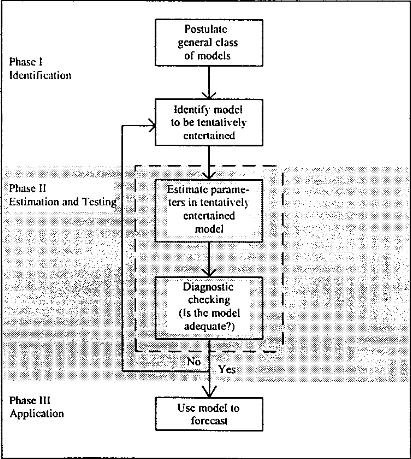
\includegraphics[width=0.4\textwidth]{Machine_learning_thesis/Images/Box_Jenkins_methodology.png}
    \caption{Schematic representation of the Box-Jenkins methodology.} 
    \label{fig:box_jenkins_methodology} 
\end{figure}

The original model used an iterative three-stage modeling approach:
\begin{enumerate}
    \item \textbf{Model Identification and Selection}: ensure the variables are stationary and identify the dependent variable's seasonality (if necessary, apply seasonal differencing). Use the plots of autocorrelation (ACF) and partial autocorrelation (PACF) functions of the dependent time series to determine which autoregressive or moving average components to use in the model.
    \item \textbf{Parameter Estimation}: utilize computation algorithms to derive the coefficients that best fit the selected ARIMA model. The most common methods for estimation are maximum likelihood estimation or non-linear least-squares estimation.
    \item \textbf{Statistical Model Checking}: test whether the estimated model conforms to the specifications of a stationary univariate process:  the residuals should be independent of each other and their mean and variance constant over time. Helpful techniques for identifying model misspecification include:
    \begin{itemize}
            \item Plotting the mean and variance of residuals over time.
            \item Performing a Ljung–Box test.
            \item Plotting the autocorrelation and partial autocorrelation of the residuals.

    \end{itemize}
    \item \textbf{Model Refinement}: if the estimation is inadequate, return to step one and attempt to build a better model.
\end{enumerate}

In empirical studies however it appears that the accuracy of such models is generally worse than much simpler time series methods. The major problem lies in the way of making the series stationary in its mean that has been proposed by Box and Jenkins. If alternative approaches are utilized to remove and extrapolate the trend in the data, ARMA models outperform the models selected through Box–Jenkins methodology \cite{Smith1997}. 

\textbf{SARIMA model}

ARIMA models do not support seasonal data, which are time series characterised by periodic fluctuations that repeats over a certain period (e.g. monthly, quarterly, yearly).
\begin{figure}[H] 
    \centering
    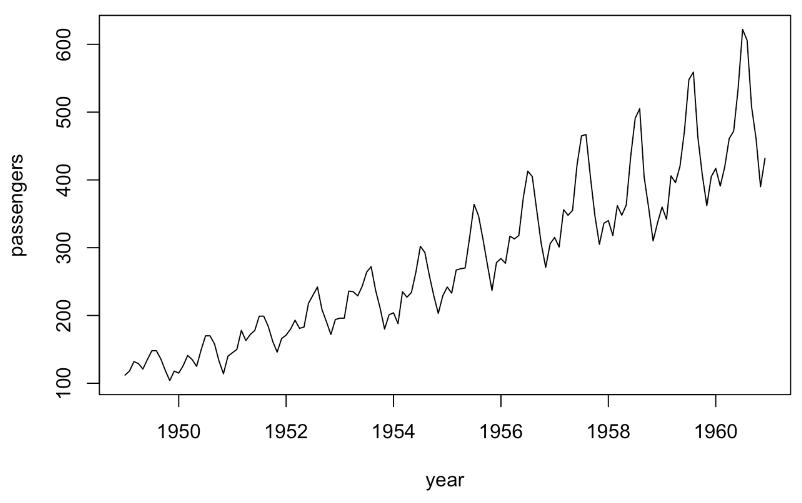
\includegraphics[width=0.4\textwidth]{Machine_learning_thesis/Images/Monthly Air Passengers(1949 - 1960).png}
    \caption{Example of a time series with seasonality (Monthly Air Passengers(1949 - 1960) Time Series).} 
    \label{fig:time_series_seasonality} 
\end{figure}
Seasonal Auto-Regressive Integrated Moving Average models, \textbf{SARIMA(p, d, q)(P, D, Q)m}, are an extension of the ARIMA (Autoregressive Integrated Moving Average) model that incorporates seasonality, by including additional seasonal terms in the ARIMA model, which are denoted by (P, D, Q)m, which represent:
\begin{itemize}
    \item P: seasonal autoregressive order
    \item D: seasonal difference order
    \item I: seasonal moving average order
    \item m: number of timesteps for a seasonal period
\end{itemize}

The general SARIMA model can be represented mathematically as follows \cite{Lee2023}:
\begin{equation}
\phi_p(B)\Phi_P(B^s)W_t = \theta_q(B)\Theta_Q(B^s)\omega_t 
\end{equation} 
where: 
\begin{itemize}
    \item \( B \): is the backshift operator, defined as \( B^k Y_t = Y_{t-k} \) 
    \item \(\phi_p(B)\): is the non-seasonal autoregressive (AR) polynomial of order p given by: \(\phi_p(B) = 1 - \phi_1 B - \phi_2 B^2 - \cdots - \phi_p B^p\)
    \item \(\Phi_P(B^s)\): is the seasonal autoregressive (SAR) component of order P given by: \(\Phi_P(B_s) = 1 - \Phi_1 B_s - \Phi_2 B_{2s} - \cdots - \Phi_P B_{Ps}\) 
    \item \(W_t\): represents the observed time series at time t. 
    \item \(\theta_q(B)\): is the \textbf{non-seasonal moving average (MA)} component of order q, give by : \(\theta_q(B) = 1 + \theta_1 B + \theta_2 B^2 + \ldots + \theta_q B^q\)
    \item \(\Theta_Q(B^s)\): is the seasonal moving average (SMA) component of order Q, given by: \(\Theta_Q(B_s) = 1 + \Theta_1 B_s + \Theta_2 B_{2s} + \ldots + \Theta_Q B_{Qs}\)
    \item \(\omega_t\): is the white noise error term at time t
\end{itemize}

\subsubsection{ARCH/GARCH}
Traditional time series models, like ARIMA models, assume costant variance over time, \textbf{homoskedasticy} \cite{MeatPrices2023}, indeed, if we look back at the formula of the ARIMA model \eqref{ARIMA equation},  \(\epsilon_t\), the white noise error term at time t is assumed to be normally distributed with mean zero and constant variance, mathematically: 
\begin{equation}
\text{Var}(\epsilon_t) = \sigma^2 \quad \text{for all } t
\end{equation}
However economic time series often shows \textbf{heteroscedasticity}, non-constant variance, that's beacuse  positive and negative news affect the variance
differently, which is known as the leverage effect. As a consequence the dispersion of residuals changes over time. 
\begin{figure}[H] 
    \centering
    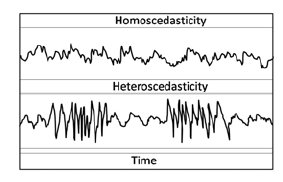
\includegraphics[width=0.5\textwidth]{Machine_learning_thesis/Images/Homoscedastic-vs-Heteroscedastic.png}
    \caption{Homoscedastic vs Heteroscedastic time series.} 
    \label{fig:Homoscedastic-vs-Heteroscedastic} 
\end{figure}

For this reason in 1982 Autoregressive Conditional Heteroscedasticity (\textbf{GARCH}) model where introduced by Robert Engle \cite{Engle1982}, to account for variance changes in financial time series by modeling the variance as a time-varying process, dependent on past errors. 









\subsection{Machine Learning for Time Series (Random Forest, XGBoost, LightGBM)} % Subsection 2.1.2
% Content for machine learning models

\subsection{Advances in Deep Learning (LSTM, GRU, CNN)} % Subsection 2.1.3
% Content for deep learning models

\section{Modern Ensemble Techniques in Time Series} % Section 2.2

\subsection{Stacking and Blending Methods} % Subsection 2.2.1
% Content for stacking and blending methods

\subsection{Recent Research on Hybrid Deep Learning Models} % Subsection 2.2.2
% Content for hybrid deep learning models

\subsection{Integrating Classical and Deep Learning Models} % Subsection 2.2.3
% Content for integrating models

\section{Gaps in Existing Research and the Need for Hybrid Solutions} % Section 2.3
\subsection{Addressing Non-stationarity and Volatility} % Subsection 2.3.1
% Content for non-stationarity and volatility

\subsection{Capturing Complex Temporal Dependencies} % Subsection 2.3.2
% Content for temporal dependencies

\subsection{The Role of Attention Mechanisms and Transformers} % Subsection 2.3.3
% Content for attention mechanisms and transformers